\chapter{Desenvolvimento do novo Portal \\FlossCoach}
\label{desenvolvimento}

O desenvolvimento do novo Portal FlossCoach foi dividido em tres fases. Na primeira, 
nós construimos um protótipo funcional com base no FlossCoach atual. Nós coneçamos o
desenvolvimento do protótipo funcional pelos motivos citados na Seção~\ref{flosscoach},
que já não atendia mais as demandas que vinha recebendo.

O objetivo desta primeira fase do desenvolvimento era que obtivéssemos como cadastrar 
os projetos com os campos para cadastro que já eram relatados no portal \\FlossCoach 
além de do cadastro de usuários.

Para a obtenção desse cadastro, tivemos algumas conversas com o Igor para que chegássemos
a um modelo de dados inicial, onde contivesse todos os itens que já estavam presentes no
FlossCoach atual e os relacionamentos que ele gostaria que huvessem entre os elementos.

\begin{figure}[h]
	\centering
	\label{fig:diagrama_iicial}
		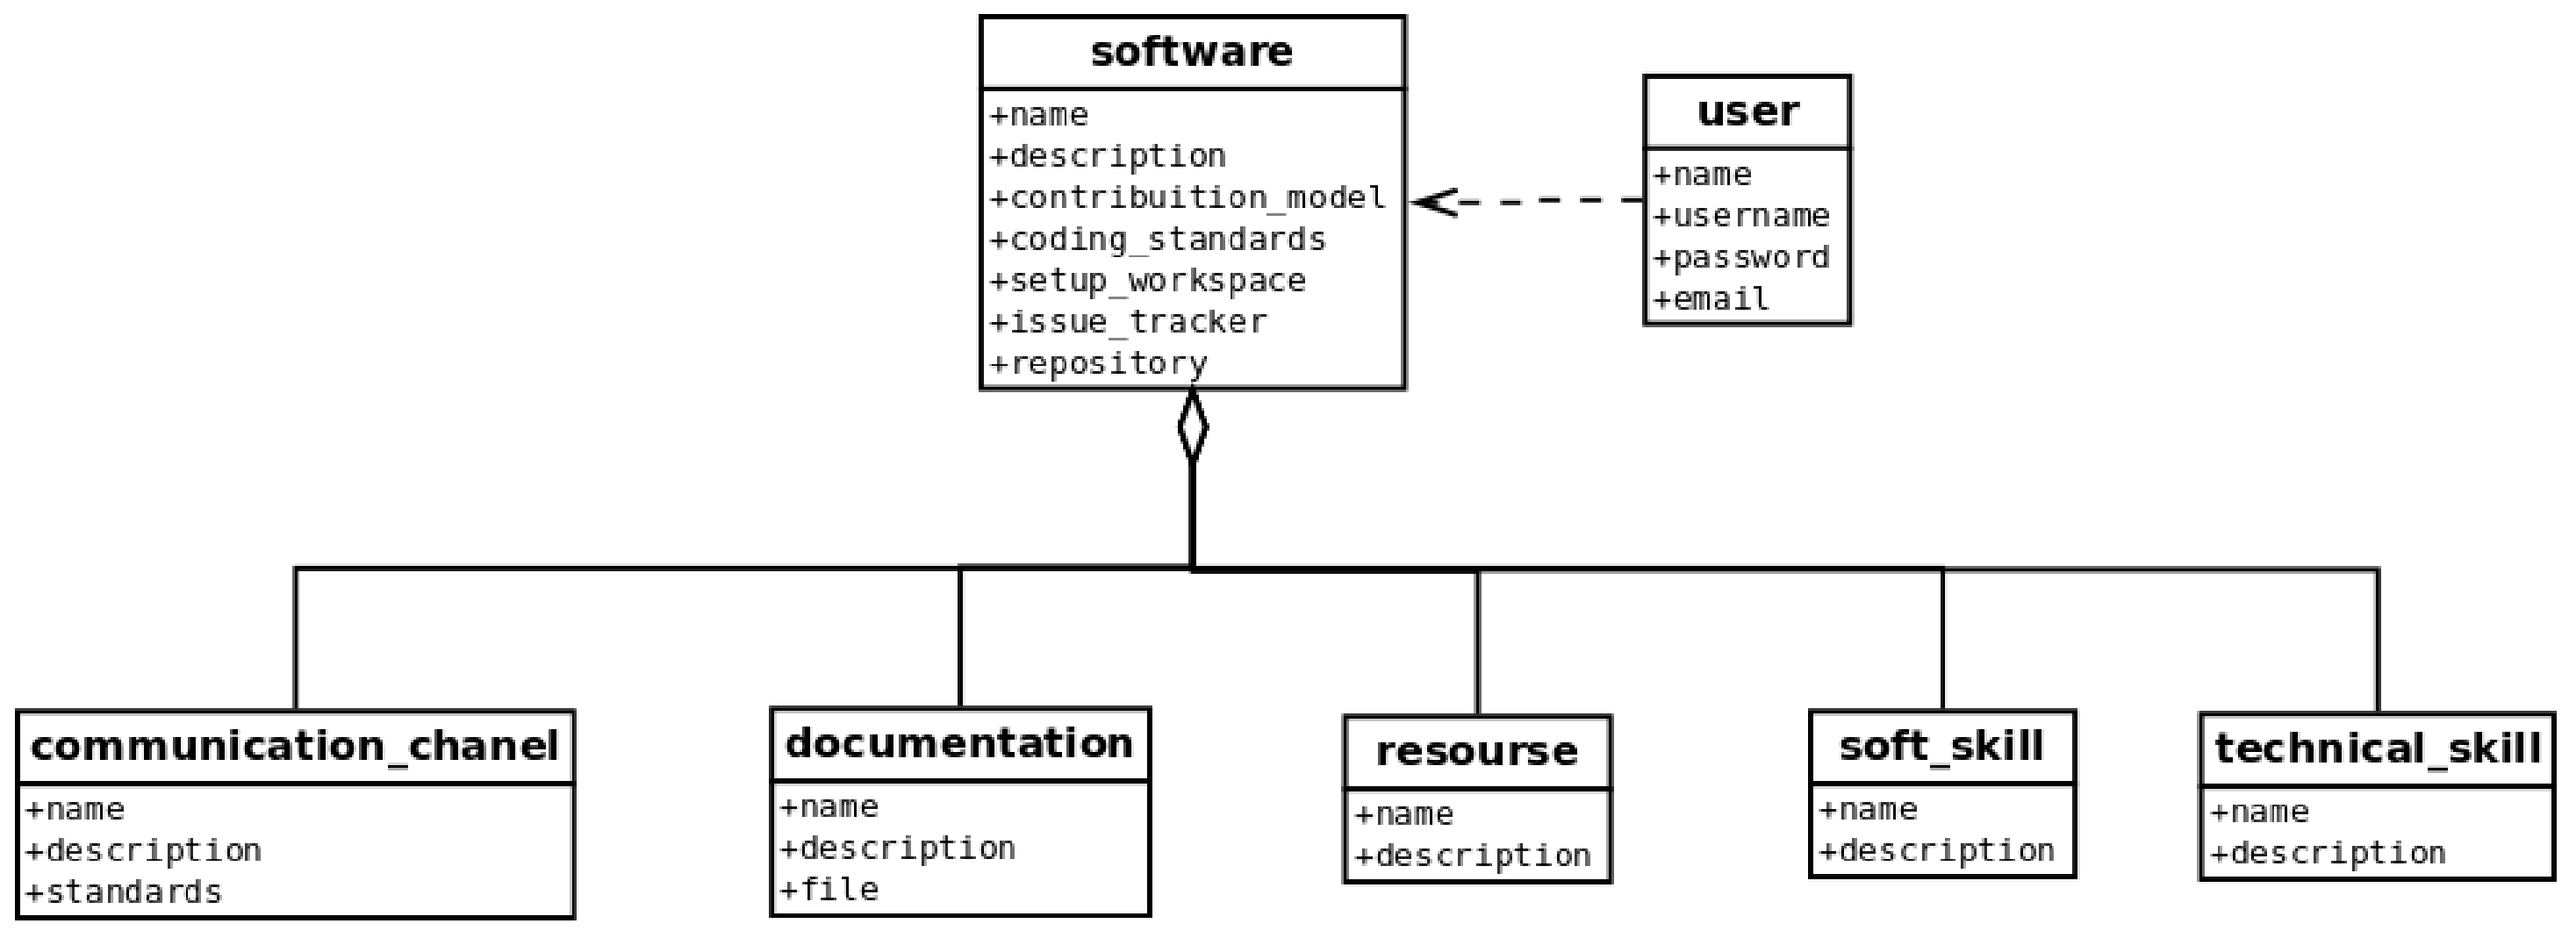
\includegraphics[keepaspectratio=true,scale=0.35]{figuras/diagrama_inicial.eps}
	\caption{Modelo de dados inicial do novo FlossCoach.}
\end{figure}

O protótipo funcional foi desenvolvido em \textit{ruby on rails} e \textit{bootstrap},
nós escolhemos estas tecnologias por serem amplamente utilizadas para desenvolvimento
de aplicações \textit{web} pela comunidade de software livre. Procuramos também utilizar
apenas de recursos de software livre para o desenvolvimento, incluindo a ferramenta de 
controle de versão e as bibliotecas utilizadas no \textit{front end}. O código da classe
software pode ser visto no Apêndice~\ref{apendice1}.

\begin{figure}[h]
	\centering
	\label{fig:prototipo}
		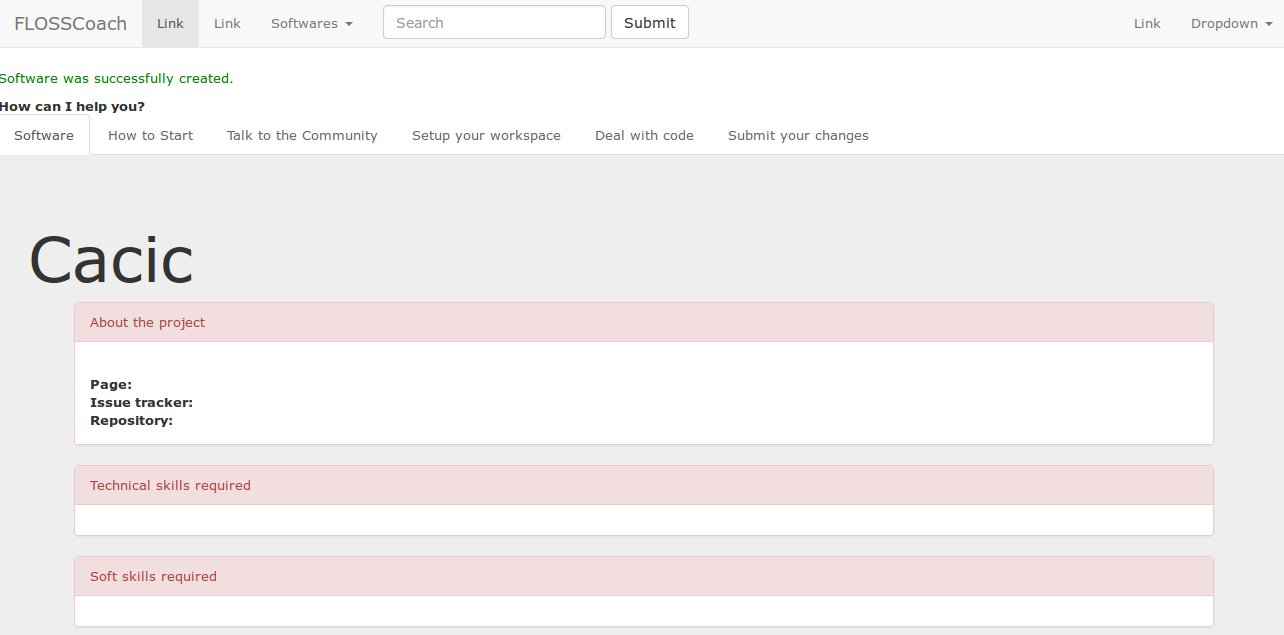
\includegraphics[keepaspectratio=true,scale=0.3]{figuras/prototipo.eps}
	\caption{Protótipo inicial do novo FlossCoach.}
\end{figure}

Esta fase do desenvolvimento durou 4 meses, iniciamos levantando os dados para implementação
em dezembro de 2015 e concluímos em março de 2016 quando nós passamos o código para o
professor Igor Steinmancher tomar conhecimento e iniciar a segunda fase do desenvolvimento.  


Na segunda fase do desenvolvimento o professor Igor Steinmancher montou uma equipe 
de desenvolvimento na USP, eles fizeram uma análise daquilo que nós havímos desenvolvido
e fizeram modificações no modelo de dados da aplicação chegando a uma segunda versão do 
modelo.

\begin{figure}[h]
	\centering
	\label{fig:diagrama_fase2}
		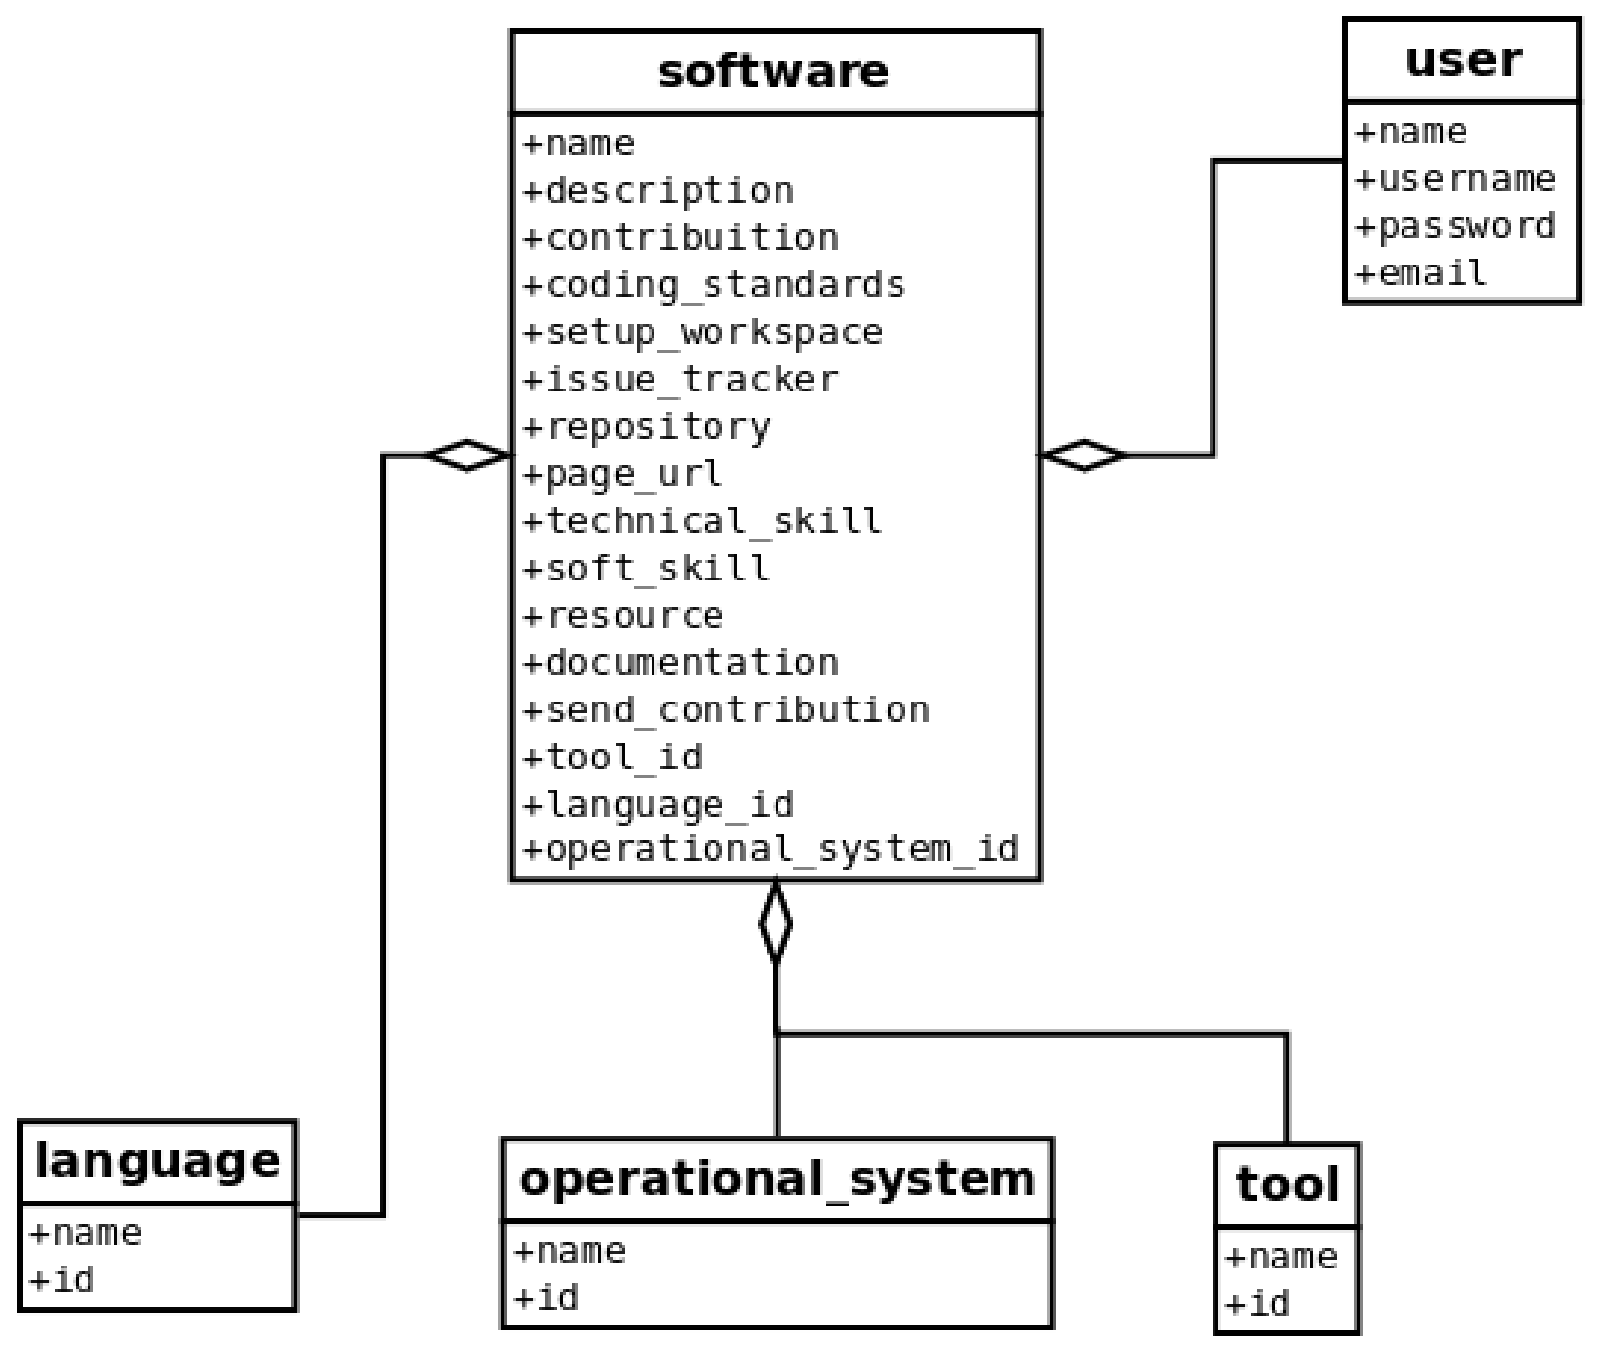
\includegraphics[keepaspectratio=true,scale=0.3]{figuras/diagrama_fase2.eps}
	\caption{Segunda versão do modelo de dados do novo FlossCoach.}
\end{figure}

Neste segunda versão no modelo de dados algumas classes deixaram de exixtir e se tornaram
atributos da classe \textit{software} e eles apresentaram 3 novas classes que não havia
no diagrama anterior. Eles implemetaram as modificações que fizeram no diagrama de dados
e melhoraram o \textit{front end} da aplicação além de desenvolver novas funcionalidades. 
Nesta etapa eles desenvolveram:
\begin{itemize}
\item Novo \textit{design} da aplicação;
\item Página de \textit{login}; 
\item \textit{Login} através de redes sociais;
\item Menu com barra lateral;
\item Modo tela cheia.
\item Consumo da API do \textit{Open hub}.
\end{itemize}

\begin{figure}[h]
	\centering
	\label{fig:prototipo}
		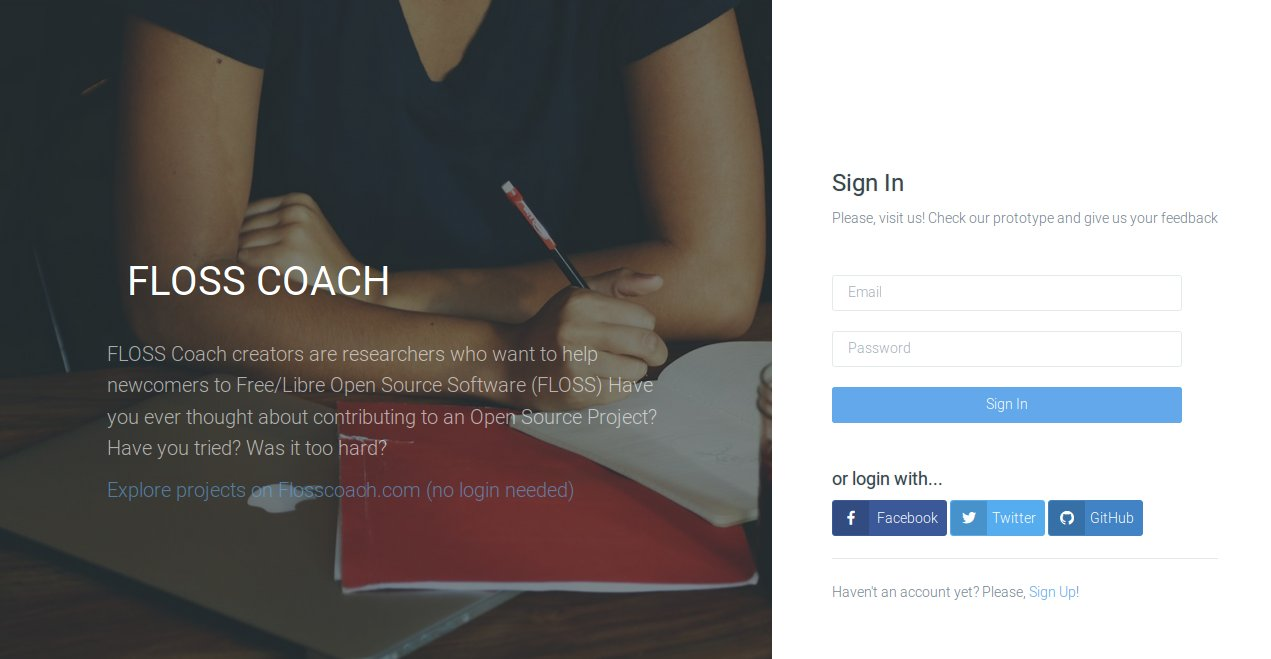
\includegraphics[keepaspectratio=true,scale=0.3]{figuras/login.eps}
	\caption{Página de \textit{login} inicial do novo FlossCoach.}
\end{figure}


\begin{figure}[h]
	\centering
	\label{fig:prototipo}
		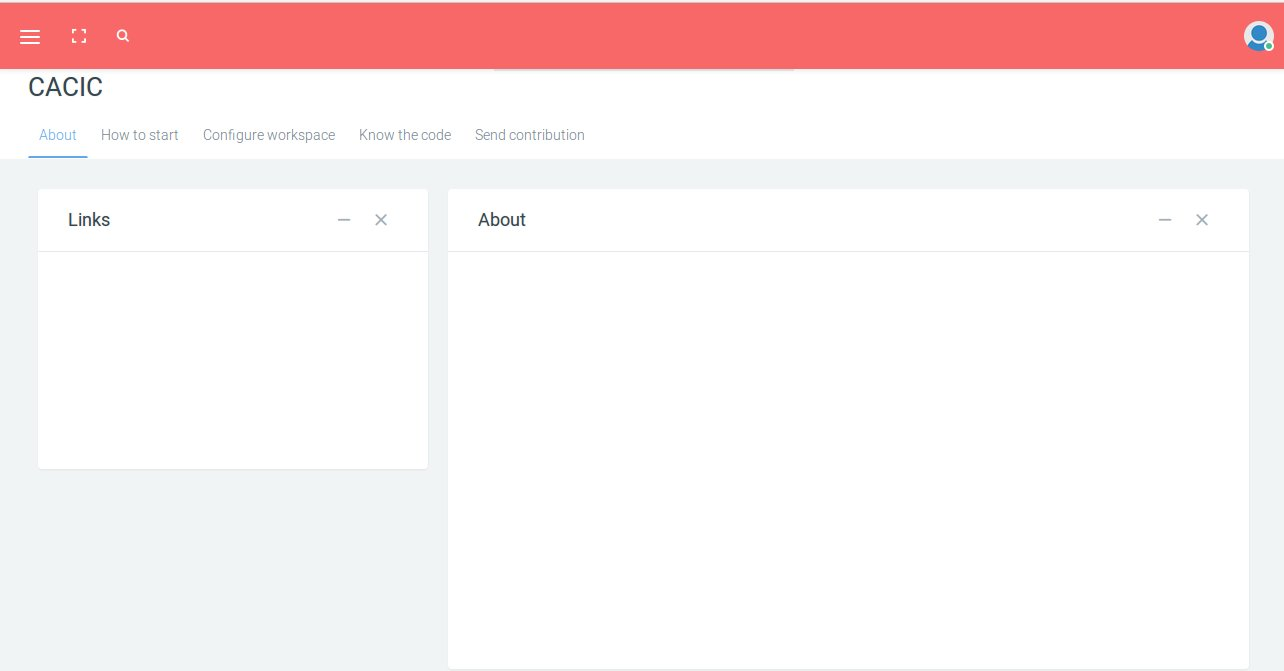
\includegraphics[keepaspectratio=true,scale=0.3]{figuras/layout.eps}
	\caption{\textit{Layout} do novo FlossCoach.}
\end{figure}


Neste intervalo de tempo da segunda fase, nós trabalhamos na pesquisa das barreiras para
contribuir com software público. Esta fase também durou 4 meses, tendo início em abril 
de 2016 e finalizando em julho de 2016.

Iniciamos a terceira fase do desenvolvimento em agosto de 2016 juntamente com a disciplina 
de manutenção e evolução de software, minitrada pelo professor Paulo Merirelles na UnB. 
Nesta disciplina os alunos escolhem um projeto que queira participar entre as opções 
dadas pelo professor e uma dessas opções foi o FlossCoach. O FlossCoach foi um dos 
projetos mais escolhidos pelos alunos e o professor Paulo teve que fazer uma seleção
dos alunos para o desenvolvimento. Após essa seleção foi montada uma equipe com
6 alunos para desenvolver o projeto.

Esta disciplina tem como objetivo aplicar técnicas de desenvolviemtno colaborativo,
são utilizados apenas projetos de software livre na disciplina para que os alunos 
possam se apropriar do código e assim fazer manutenções corretivas e evolutivas no
mesmo.

Para a organização da disciplina e evolução dos alunos, o desenvolvimento é dividido
em \textit{sprints}, quase sempre de duas semanas, como mostrado na Figura~\ref{fig:disciplina}
onde são aplicadas as práticas de desenvolvimento ágil. No início de cada sprint é feito um planejamento da sprint, 
onde são escolhidas as \textit{issues} que serão desenvolvidas naquela \textit{sprint}.
No início da aula é feito um \textit{stand up}, uma reunião em pé, de no máximo 15
minutos para que seja passado para os outros membros da equipe o \textit{status} da
tarefa o qual está responsável e ao final da sprint é feita uma revisão da \textit{sprint},
momento para fechar as \textit{issues} que foram concluídas na \textit{sprint}, 
analisar as que não foram concluídas e apontar os motivos afim de que os outrs membros
da equipe possam ajudar.

Para que uma \textit{issue} seja aceita criamos uma política de que deveria ter
testes unitários para o que fosse implementado além de que os testes já existentes
deveriam estar funcionando, como no exemplo de código no Apêndice~\ref{apendice2}.
No início desta fase de desenvolvimento houve uma preocupação 
em criar testes unitários do que já havia sido implementado no FlossCoach pois 
não havíamos tido essa preocupação anteriormente. Era necessário também que outro 
membro da equipe revisasse o código e o aprovasse para que feita a revisão final
por mim, que tinha permissão para acoplar ou não àquele trecho de código ao
código oficial. 

No FlossCoach eu acompanhei todas essas práticas juntamente com a equipe e estava
a disposição para que os alunos da disciplina pudessem tirar dúvidas. Foram desenvolvidas
6 \textit{sprints} ao longo do semestre cujas \textit{issues} desenvolvidas podem
ser vistas na Tabela~\ref{issues}.

A \textbf{Sprint 1}, foi planejada para que os alunos pudessem levantar o ambiente
do FlossCoach em suas máquinas além de estudar o código e suas funcionalidades. Com o
ambiente funcionando corretamente em todas as máquinas, nós configuramos uma ferramenta
para o desenvolvimento de testes unitários chamada \textit{rspec}, e iniciamos o 
desenvolvimento de alguns testes das \textit{models} do FlossCoach. 

Na \textbf{Sprint 2}, planejamos a criação de um papel de administrador aos usuários
e a atribuição deste papel ao usuário que cria um novo projeto além de aprovar 
membros para serem administradores do projeto. Nesta etapa todos os usuários podem
modificar os projetos e a criação do papel de administrador é a primeira tarefa 
para que outros usuários deixem de poder modificar os projetos. Foram feitas a 
criação e atibuição do papel de administrador ficando faltando os testes que
ficaram como dívida técnica para a próxima \textit{sprint}, e não tivemos tempo para fazer a 
aprovação de membros. 

Para a \textbf{Sprint 3}, pensamos em configurar a internacionalização do FlossCoach
devido à pesquisa com softwares públicos, além de adicionar nosvos campos ao cadastro 
de usuário que foram pensados juntamete com o Igor para deixar o cadastro de usuário 
mais completo e o conserto de um link quebrado para a página de perfil de usuário.
Também fizemos os testes da criação e atribuição de papel de admintrador ao uauário
que cria o projeto concluindo assim todas as tarefas planejadas para a \textit{sprint}.

A \textbf{Sprint 4} foi planejada para que fosse uma \textit{sprint} individual, que
significa que cada membro do grupo resolverá uma issue sozinho, dessa forma foram 
planejadas tarefas mais simples para que cada um consiga concluir ao menos uma
tarefa na sprint, dessa forma planejamos a internacionalização da \textit{homepage},
página de projetos, página de perfil de usuário e cadastro de usuário alem da 
tarefa de permitir que usuários possam editar seu perfil e corrigir um erro que
estava ocorrendo no cadastro de um novo usuário que sempre dizia que o email já
estava cadastrado mesmo efetuando o  cadastro. Como as tarefas eram simples,
alguns membros terminaram suas tarefas antes do final da \textit{sprint}, eles 
pegaram outra tarefa para fazer.

\begin{table}[h]
	\centering
	\begin{tabular}{ccc}
		\toprule
		\textbf{Sprint} & \textbf{Issues desenvolvidas} \\
		\midrule
		Sprint 1 & Levantar ambiente e tomar conhecimento do FlossCoach \\
			 & Configurar ambiente de testes unitários \\
			 & Iniciar testes das \textit{models}\\
		\midrule
		Sprint 2 & Criar papel de administrador do projeto\\
			 & Atribuir papel de administrador ao usuário que cria o projeto \\
			 & Aprovação de membros em projetos \\
		\midrule		
		Sprint 3 & Configuração da internacionalização \\
			 & Adicionar novos campos ao cadastro de usuário\\
			 & Redirecionar o \textit{link} de perfil para a página de perfil do usuário.\\
			 & Testes de papel de administrador.\\
		\midrule		
		Sprint 4 & Traduzir \textit{homepage}.\\
			 & Traduzir página de projetos.\\
			 & Traduzir página de perfil de usuário\\
			 & Traduzir cadastro de usuário.\\ 
			 & Permitir usuários a editar o seu perfil\\
			 & Corrigir erro de cadastro de e-mail já registrado.\\
			 & Estudar uma \textit{gem} de sistema de \textit{loging}.\\  
		\midrule		
		Sprint 5 & Inserção de campos específicos para software público.\\
			 & Implementar rotina de esqueci minha senha.\\
			 & Colocar barra de internacionalização em todas as páginas.\\
			 & Impedir criação de projetos com mesmo nome.\\
		\midrule
		Sprint 6 & Configurar \textit{gem} de campos customizáveis.\\
		\bottomrule
	\end{tabular}

	\caption{Conteúdo das sprints da terceira fase do desenvolvimento.}
	\label{issues}
\end{table}


